\chapter{The role of introgression in the adaptive evolution of the generalist plant pathogen, \textit{Albugo candida}}
\label{chap:Acandida}
\chaptermark{Evidence of hybridisation in \textit{Albugo candida}.}

This chapter is based on the published scientific paper:

\vspace{5mm}

\textit{McMullan, M., Gardiner, A., Bailey, K., Kemen, E., Ward, B. J., Cevik, V., ... Jones, J. D. (2015). Evidence for suppression of immunity as a driver for genomic introgressions and host range expansion in races of Albugo candida, a generalist parasite. eLife, 4, 1-24.}

\vspace{5mm}

This thesis chapter presents a research project that was a collaboration between many researchers.
In this chapter in order to provide clear description of the work involved, some details regarding some work that has not been performed by myself are presented.
Specifically, work described in sections 3.2.1 and 3.2.2 were completed by collaborators and not myself.
My contributions to the work are described in sections 3.2.3 and 3.2.4, and it is results of this work that is presented in this chapter.


\newpage


\section{Introduction}
Host specificity is a defining feature of pathogens, and can be defined as the inverse of the number of hosts that a given pathogen can infect \parencite{Poulin2008}. Host specificity is negatively correlated to the probability of parasite extinction, and positively correlated to the ability of a parasite to colonise and adapt to a new host \parencite{Poulin2008}. Host specificity is constrained by the physiology of the pathogen. Therefore the host specificity of a pathogen is constrained by factors including (but not limited to) the pathogen's method of transmission, method of obtaining nutrients and energy from the host, and the ecology of the pathogen and host \parencite{poulin2011evolutionary}. Such factors are proximal constraints on host specificity, but host specificity is ultimately constrained by the evolutionary and biogeographical history of the pathogen and its potential hosts \parencite{Poulin2008,poulin2011evolutionary}.

A highly specialist parasite occurs in only a single host species. They often require host-host contact for transmission, and their longevity and future is strongly linked to that of their host species \parencite{Poulin2008}. Conversely, a parasite that is more generalist may survive the extinction of one host species, since there is another host species they can exploit to survive. Generalist parasite species may rely less on contact-transmission or close proximity between hosts. For example, they may be transmitted through food, or some other species vector \parencite{Pedersen2005PatternsPrimates}. However it should be noted that even if a pathogen has a very high mobility, and dispersal, its host-specificity can be high \parencite{Poulin2008}.

The availability of ecologically and evolutionarily related or similar hosts cohabiting the same habitat, may cause differences in the host-specificity of two otherwise similar pathogen species \parencite{Jex2006TheSpecificity.}. Furthermore, parasites put selective pressure on host populations to adapt and develop immunity, increasing the frequency of genetic and epigenetic variants that improve immunity, and pathogen detection in the host. As a result, these adapting host populations impose selection pressure on the pathogen populations, increasing the frequency of variants that maintain the pathogens efficiency of immune suppression. Over time, both host and parasite co-evolve and become intimately associated, as they both adapt to each other's latest antagonistic evolutionary innovations. This is called an evolutionary arms-race \parencite{Boutemy2011,Buckling2002,Cooper2008,Kemen2012,Lamour2010}.

Overall, the general pattern observed in nature, is that most parasite species are largely specialised and co-evolve with only a few, if not one, host species \parencite{McMullan2015a}. It should be noted however, that this generalisation is based on a measure of host specificity that is based on a simple measure of host specificity, namely the number of host species that are colonised by a parasite in natural populations. However this metric makes an oversimplification that does not reflect biological reality. For example, two pathogen species may have the same number of host species, but if one of the pathogens infects species of one genus, and the other infects species of multiple genera, then it is not realistic to conclude both of the parasite species are equally specialised. It is because of this problem, that \cite{Poulin2003ParasiteSpecificity} defined a host-specificity measure that takes into account the taxonomic or phylogenetic distances between the hosts colonised by a parasite. Later the authors published an improved metric that incorporated the phylogenetic or taxonomic distinctness of a pathogens host species, but also weighted for the prevalence of the parasite on its different host species \parencite{Poulin2005CombiningSpecificity.}⁠. The rationale for such a weighting is that a pathogen that is largely concentrated on only one of its multiple hosts should be classified as more specialised than a pathogen that utilises and colonizes all of its host species evenly.

The organism of interest in this work is the obligate biotrophic plant pathogen, \textit{Albugo candida}. Plant pathogens have a parasitic relationship with their host, and are classified according to the nature of this relationship with the host. Pathogens which obtain nutrients from decaying plant matter are classified as necrotrophs, whereas pathogens which require living host tissue in order to obtain nutrients are classified as obligate biotrophs \parencite{Kemen2012}⁠. These biotrophs don't typically secrete abundant lytic enzymes, and cause little physical or structural damage to the host plant \parencite{Kemen2012}⁠. Pathogens with a combination of these two lifestyles are classified as hemibiotrophic \parencite{Kemen2012,Lamour2012PathogenCapsici}. \textit{Albugo candida} is an obligate biotroph, and whilst \textit{Albugo candida} is a generalist, infecting species of the Brassica family, obligate biotrophs are typically specialists \parencite{McMullan2015a}⁠.

After an obligate biotroph makes a host-jump, it is expected that selection will increase any adaptive genetic or epigenetic variant in the population that results in more efficient immune suppression of the new host \parencite{Dong2014,Kemen2012,Poulin2008,Raffaele2010,Thines2014}. Furthermore, host-parasite co-evolution over time will result in both the host and parasite constantly adapting to each others latest antagonistic adaptations, and they will become more intimately associated historically \parencite{Morgan2007,Raffaele2012,Thines2014}. As both of these processes occur, new effectors and pathogenicity factors may be created, and existing ones may receive beneficial mutations, and they may also have their levels of expression changed epigenetic modification and inheritance \parencite{Dong2014,Gijzen2014EpigeneticPathogens,Raffaele2012,Raffaele2010,Win2012}. These will be fixed due to selection pressure if they are beneficial. These modifications enable more efficient immune suppression and exploitation of one host species, but increase the risk of detection in other host species by triggering their immune system \parencite{Martin2012EffectorsInteractions}. Thus, as obligate biotrophic pathogen populations become more adept at suppressing the immunity of one host, they will become less adept at infecting previous host(s) or other hosts it can infect.

Therefore, obligate biotrophs are typically known for being intimately associated with their hosts i.e. they have a high host specificity \parencite{Thines2014}. Yet there are generalist biotrophic parasites that appear to have overcome this evolutionary dilemma and show virulence on diverse hosts. \textit{Albugo candida}, the organism that is the subject of this work, is one such generalist, but there are other generalist oomycetes, like \textit{Phytophthora capsici} \parencite{Lamour2012PathogenCapsici}⁠.

Some generalist parasite species have solved the dilemma by evolving multiple specialised races, and each specialised race can infect a different host. For example, the eukaryotic order \textit{Albuginales}, of which \textit{Albugo candida} is a member, is completely comprised of obligate biotrophic pathogens that cause disease on a broad range of plant hosts \parencite{Biga1955ReviewConidia.,Choi1955,Walker2007AHost.}.

Albugo is the largest genus of the order \textit{Albuginales}, and it was reported to consist of 33 specialist pathogens by \cite{Biga1955ReviewConidia.}⁠. More recently, the estimate is that the genus comprises approximately 50 pathogens, and these are typically specialists. In addition new distinct \textit{Albugo} species have been discovered that were previously thought to be members of \textit{Albugo candida} (Pers) Roussel. \parencite{Choi2011,Choi2009,Ploch2010,Thines2009}. This is because in the past decades, classification was based largely on morphology, and this led to the application of a broad species concept, that resulted in \textit{Albugo candida} (Pers.) Roussel being regarded as the causal organism of all incidents of white blister rust on all \textit{Brassicaceae} hosts \parencite{Choi2011}. As late as 2011, it has been estimated that “a dozen” distinct species thought to be \textit{Albugo candida} await discovery \parencite{lamour2009oomycete}.

\textit{Albugo candida} (Pers.) Roussel can infect 241 species of plants in 63 genera from the families of \textit{Brassicaceae}, \textit{Cleomaceae} and \textit{Capparaceae} \parencite{Choi2009}⁠. \textit{Albugo candida} infections are the causal agent of white blister rust disease, resulting in significant losses on \textit{Brassica} crops of economical importance. For example, \textit{Albugo candida} causes  up to 56 of yield losses in Indian Mustard \parencite{Meena2002YieldSeverity}. \textit{Albugo candida} consists of different “physiological races”, each usually featuring high host-specificity and approximately 24 races of \textit{Albugo candida} have been defined, based on their host range \parencite{saharan2014white,Saharan1992WhiteSpecies}.

\textit{Albugo candida} reproduces both asexually and sexually \parencite{Holub1995}⁠. During asexual reproduction, diploid zoospores are formed in zoosporangium beneath the leaf epidermis. The zoosporangium are visible when dehydrated and in large numbers, as white blisters \parencite{Holub1995}. These sporangia then rupture the epidermis of the host leaf, to release zoospores for dispersal. During sexual reproduction, fertilization between two isolates creates non-motile, diploid, and thick-walled oospores \parencite{Holub1995}⁠. The oospores can resist extreme temperatures and desiccation. The relative importance of both reproductive modes is not well established, but the clonal (asexual) mode of reproduction allows rapid population expansion, especially given modern crop mono-culture growing practices. Although \textit{Albugo candida} comprises distinct, specialised physiological races that colonize different host plants, and that distinct species have been identified that were initially thought to be \textit{Albugo candida} \parencite{Choi2011}, it is still considered a single species.

According to evolutionary and population genetic theory, the trade-offs associated with adaptation and host-specialisation, coupled with strong population structuring, can result in adaptive radiation and speciation \parencite{Abbott2013,Stukenbrock2013EvolutionPathogens}. \textit{Albugo candida} then may be thought of as a currently ongoing adaptive radiation; The broad host range of \textit{Albugo candida} is enabled by an ongoing specialisation of independent physiological races, and these races are likely heading for speciation \parencite{Dres2002a}. If strains or races of a parasite develop adaptations to specific hosts, and make trade-offs in doing so, specialising to the given host, does parasite specialization inevitably lead to speciation? Certainly, specialising on one or a few hosts, at the cost of being able to infect other hosts, will mean separation of specialised races, ecologically, and even geographically, over time such separation is expected to result in  reproductive isolation.

Compared to other microbial plant pathogens, \textit{Albugo} species are notable as infections strongly suppress host innate immunity. As a result, infections of \textit{Albugo} species increase the susceptibility of the host to a secondary infection by pathogens that would otherwise be avirulent, including downy mildews \parencite{Cooper2008}. It has been suggested that this immune suppression caused by \textit{Albugo} infections might allow an accelerated adaptation of other pathogen species to host that is susceptible to \textit{Albugo} species \parencite{Thines2014}⁠.

However, whilst it has been suggested the immune suppression will accelerate the adaptation of other pathogens to the suppressed host, before this project, no evolutionary rationale was proposed explaining why rendering a host susceptible to other pathogens could be adaptive for the various Albugo species. Hypothetically, a pathogen which colonizes and adapts to the hosts of Albugo species due to the immune suppression of Albugo species infections, will become competition against Albugo species for the same resources \parencite{Cooper2008}⁠.

Suppression of host innate immunity would facilitate cohabitation of distinct physiological races that otherwise would not come into contact due to their specialisation and adaptive trade-offs, as previously discussed. When the distinct physiological races come into contact, genetic exchange including introgression and hybridisation may occur between them. Here, introgression is defined as the introduction of nucleotide variation from a parental donor race into the genome of a recipient race, through the mechanism of recombination \parencite{Hedrick2013}. This flow of genetic variation from one donor physiological race, to a recipient physiological race, could slow down the genetic divergence of the races, and slow or prevent speciation. However, introgression between races that are specialised and adapted to exploit different hosts could be maladaptive, and therefore could be strongly selected against. This is because hybrids would inherit effector alleles derived from both parental races. Therefore, whilst the hybrid genomes would contain effectors that enable the immune suppression of multiple hosts, they could also contain effectors that trigger immunity on multiple hosts. Immune recognition of even a single effector is sufficient to trigger the immune response and stop an infection. Therefore any hybrid that possess an expanded repertoire of effector alleles are likely to have a strong fitness disadvantage on most potential host plants, as with larger effector repertoire's comes an increased likelihood of one of them triggering host immunity.

This chapter presents work conducted and contributed to a larger genome project analysis of \textit{Albugo candida}, conducted by a team of scientists at the University of East Anglia, and The Sainsbury Laboratory. This project aimed to answer the following questions, in order to try and resolve this question of whether immune suppression and secondary infection is adaptive or maladaptive, and whether it is due to hybridisation:

\begin{enumerate}
\item Are the distinct physiological \textit{Albugo candida} races genetically isolated and ‘on the road to speciation’?
\item Does suppression of host innate immunity enable cohabitation and growth of races with non-overlapping host ranges?
\item Are the genomes of \textit{Albugo candida} affected by recombination and hybridisation?
\end{enumerate}

The work presented in this chapter was primarily conducted with a goal of answering the third question of the project. During the collaborative project, genome sequence assemblies were created for five isolates that were collected from four host species (\textit{Brassica oleracea}, \textit{Brassica juncea}, \textit{Capsella bursa-pastoris}, and \textit{Arabidopsis thaliana}). This chapter presents analyses performed on the assembled sequence scaffolds for the detection of recombination, hybrididation, and mosaic genome structure.


\section{Methods}
In order to perform the analysis of genome structure that is the focus of this chapter, prior work was conducted to isolate the \textit{Albugo candida} races used in this study, test for virulence, extract and sequence DNA, and RNA, and perform genome and transcriptome assemblies. These procedures are subsequently described in detail in \parencite{McMullan2015a}, and given that these procedures are not the focus of this chapter, the reader is referred to this paper for details on the wet lab and molecular methods. A brief summary of these methods is described below.

\subsection{Isolation and cultivation of races used in the study}
In order to address the research questions presented in the previous section, genome sequence assemblies were required of five isolates of \textit{Albugo candida}, the white rust fungus. These isolates were collected from four different host species: \textit{Brassica oleracea}, \textit{B. juncea}, \textit{Capsella bursa-pastoris}, and \textit{Arabidopsis thaliana}. The isolates were collected by Erik Kemen, prior to the evolutionary analyses that are the focus of the present chapter. 

The isolate designated AcNc2, was isolated from infected leaves of \textit{Arabidopsis thaliana} Eri-1 field-grown plants in Norwich, England. The isolate was collected in 2007. The isolate AcEm2 was collected from wild \textit{Capsella bursa-pastoris} in Kent, England in 1993. AcBoT was collected from infected cultivars of \textit{Brassica oleracea} called 'Bordeaux F1', from Lincolnshire, England, in May 2009. AcBoL was harvested from infected \textit{Brassica oleracea} leaves from Lincolnshire, but in the January of 2009. An isolate which is virulent on \textit{Brassica juncea} called Ac2V was provided by M Borhan of Agriculture and Agri-Food, Canada. All of these isolates were single spore purified \parencite{Kemen2011}.

\subsection{Genome assemblies of isolates}
The assembly of isolate AcNc2 was used as a reference. The assembly is 34Mb in size, and has 5212 contigs of approximately 160-fold coverage. The assembly was approximately 73\% of an estimated genome size of 45Mb. The unassembled part of the genome (approximately 11Mb) is likely to contain repeats, approximately 8\% of which represent collapsed regions, since they have coverage that is several times higher than the average. For each isolate, several assemblies were constructed with different k-mer lengths. Each assembly was assessed according to number of contigs, N50 (Bp and number), mean contig length, assembly size, GC content, average genome coverage, repeat content, and the number of predicted genes. High sequence similarity of the five \textit{Albugo candida} isolates resulted in the conclusion that three races had been sequenced: AcNc2, and AcEm2 were isolates of the same race, and AcBoT and AcBoL were also two isolates which belonged to the same race. Therefore, detection of recombination and hybridisation in this chapter were first conducted on the three races AcNc2, Ac2V, and AcBoT, each of which had a 33-34Mb assembly.

\subsection{Detection of recombination events}
Recombination events were statistically identified on contigs $\geq$10,000 Bp using the software RDP3 using five independent detection algorithms: RDP \parencite{Martin2000RDP:Sequences.}, GENECONV \parencite{Padidam1999PossibleRecombination.}, Maxchi \parencite{Smith1992a}, Chimaera \parencite{Posada2001b}, and 3Seq \parencite{Boni2007AnTriplets}. All of these tests are available in the Software Package RDP for Microsoft Windows \parencite{Martin2015RDP4:Genomes}. Tests were conducted using a critical value α = 0.05 and p-values were Bonferroni corrected for multiple comparisons of sequences. Sequences were made linear using unphased base calling, i.e. where a sequence has a base position that is heterozygous, one of the nucleotides was assigned at random at that site. 

Recombination events were only considered genuine if they were supported by at least three of the recombination detection methods in RDP, and recombination events detected using the methods in RDP were only counted if the parental sequences could be identified, and the start and end positions of recombination events were unambiguous.

In order to visualise the effects of recombination and hybridisation on the genome structure of the \textit{Albugo candida} races, the software package HybridCheck was developed for the R programming language. The development and testing of this software package is described in detail in chapter \ref{chap:HC}, so only a brief description will follow. HybridCheck can analyse three sequences with a sliding window scan, and produce plots with use the RGB tricolour system to indicate where regions of hybridisation or recombination have occurred between sequences. Each sequence is designated one of the three primary colours, red, blue, or green. In regions of a given sequence that are unique, then those regions are coloured in with the unique colour of that given sequence. However, in regions of the sequences in which all the SNPs are shared with another sequence, then the region is coloured with the “hybrid” colour of the two sequences (e.g. yellow if the two sequences have the unique colours red and green). All monomorphic sites are excluded in this computation. In cases where recombination is recent, the hybrid colouration is strong as most of the SNPs are shared between two sequences. However older events may have accumulated mutations since the recombination / hybridisation event. In such a case, there are less shared SNPs between two sequences, and the colour intensity is less strong.

\subsection{Dating identified recombination events}
Immediately after a recombination or hybridisation event has occurred, a hybrid or recombinant offspring's DNA sequence will have regions which are near identical to one parent, and regions which are near identical to the other parent. In those regions the molecular clock is effectively zeroed. Therefore, for a given recombinant region, the only substitutions which could be observed between the recombinant and the donor must have occurred since the recombination event took place.

This divergence between a donor sequence region, and the same region in the recombinant offspring was used to estimate the time since the recombination event. Two methods were used to calculate the number of generations since individual identified recombination events occurred. A binomial mass function was used, which was developed for the HybridCheck R package. The equations are described more fully in chapter \ref{chap:HC}. Briefly, the method computes a window of time, within which the recombination event is most likely to have occurred. It does this by taking into consideration the cumulative probability of observing the number of mutations that have occurred in the recombinant region, between donor and parent, given the average mutation rate. The function assumes that the recombination event has evolved neutrally since the recombination event occurred, and that mutation rates between the two sequences were constant through time, and equal in both sequences. The mutation rate in oomycetes is unknown, and therefore the binomial mass function was used with two different mutation rates: μ = 10−6 and 10−7 per base per generation. This binomial mass function was used to analyse all detected recombination events.

In addition to the binomial mass function, an analysis was conducted in BEAST \parencite{Drummond2007BEAST:Trees}. Phylogenetic trees were estimated with a HKY + G model, a Yule tree prior, and a strict molecular clock assumption, where the mutation rate was assumed to be $\mu = 10^{−6}$. Ten independent analyses were run, with an MCMC of 10 million steps, with a burn-in of 10\%. Because of the computational complexity and time required for BEAST analyses, 20 recombinant regions were analysed in this manner. The results were compared to the date that was estimated for the recombinant region by the binomial mass function, and this confirmed that the binomial mass function provides a good approximation of the divergence time.


\section{Results}
\subsection{Distribution of polymorphisms across races}
Polymorphisms were found to be unequally distributed across the genomes of the \textit{Albugo candida} isolates analysed. In some regions of the genome, there are stretches of identical sequence which are as long as 10kb in length. In other regions of the genome, stretches of lower sequence similarity may be found. For example, between the isolates AcBoT and AcNc2, a region of approximately 5kb was observed with 89\% sequence similarity. This is demonstrated in Figure \ref{fig:AC_Res_1}.

\begin{figure}
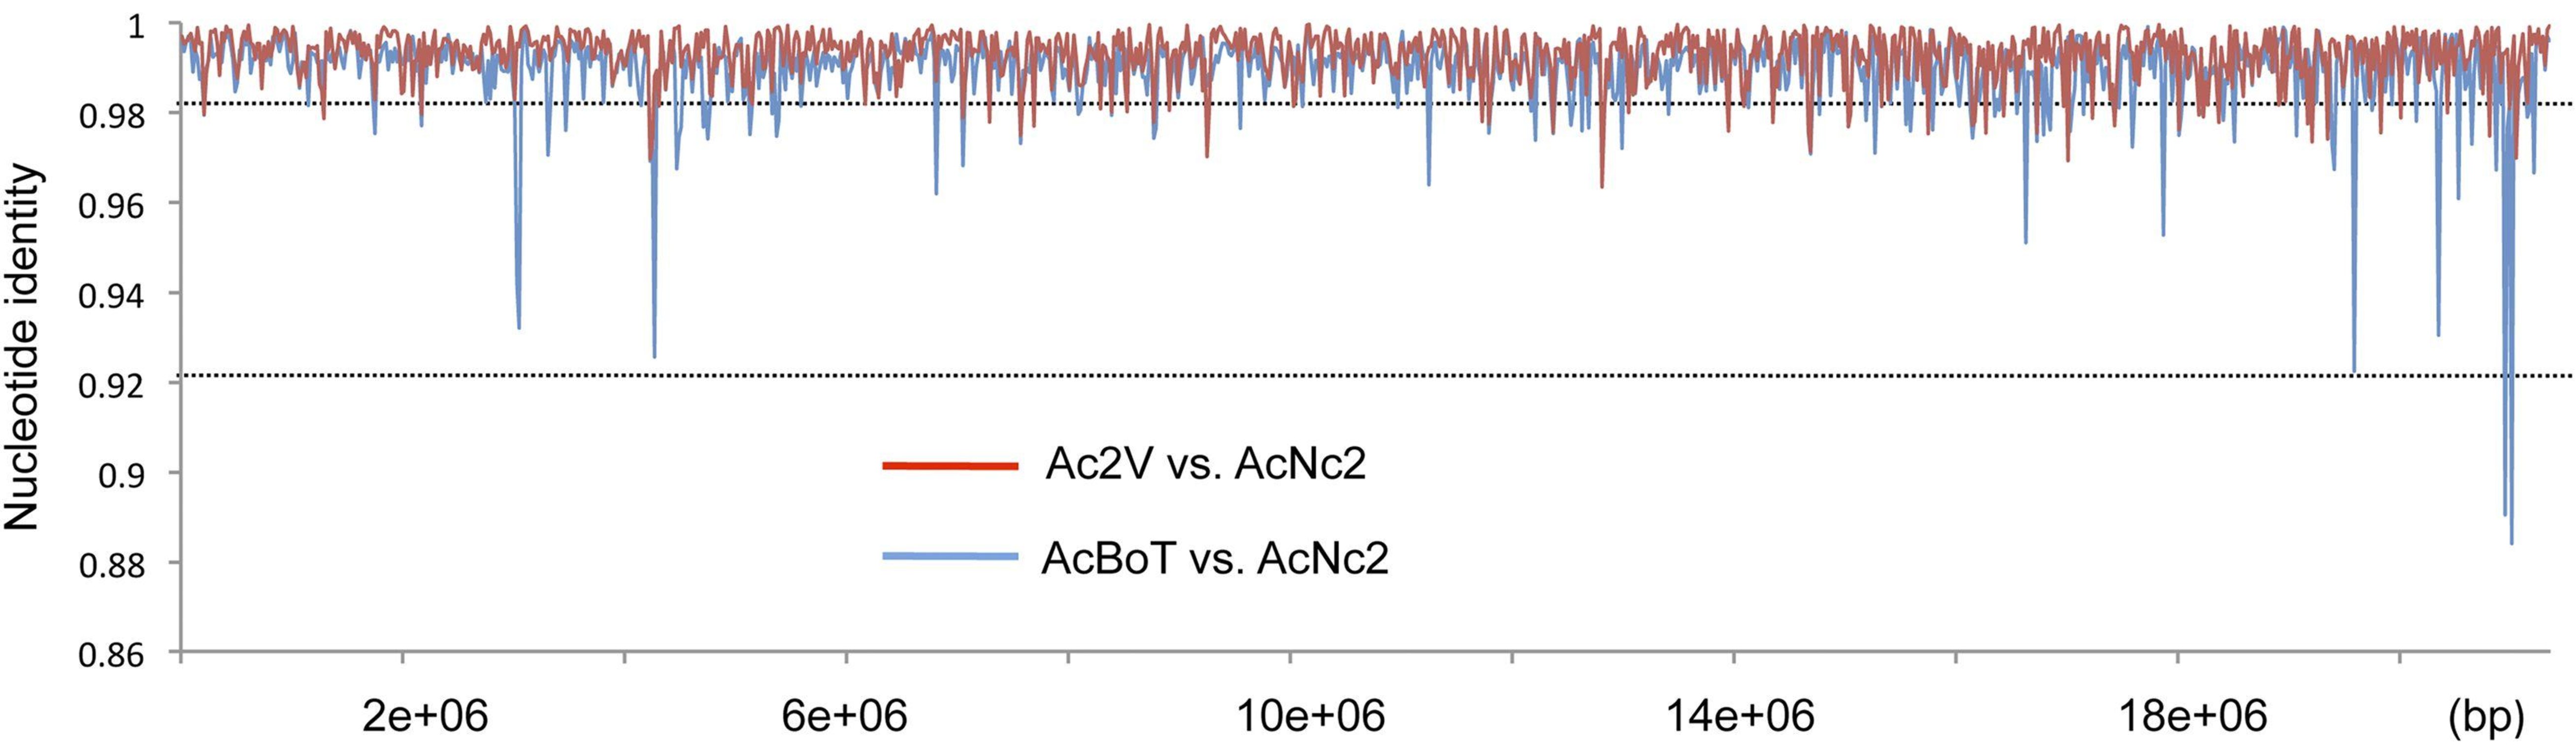
\includegraphics{Figures/AlbugoCandida/AC_Figure1}
\caption{Nucleotide identity amongst the homologous genomic regions of Ac2V, AcBoT and AcNc2. The mean identity was calculated for the sliding window of 20 Kb.\label{fig:AC_Res_1}}
\end{figure}

The distribution of the polymorphisms is highly suggestive of a mosaic-like genome as the polymorphisms are not only distributed unevenly, but they were distributed in a block-like manner.
Stretches of nucleotide similarity are arranged in a block like structure; there are regions where AcNc2 is highly similar to AcBoT (and therefore diverged from isolate Ac2V), followed by regions where isolate AcNc2 is highly similar to Ac2V (and therefore diverged from isolate AcBoT).
The HybridCheck software package visualises such genome structure in Figure \ref{fig:AC_Res_2}. The figure visualises the effect on the genome by colouring regions yellow where races AcNc2 and AcBoT show near sequence identity, cyan where races AcBoT and Ac2V show near sequence similarity, and purple where races AcNc2 and Ac2V show near sequence similarity.
Note that in the figures, there are also regions of unique colouration (red, green, and blue), and such regions represent diverged parts of the genome where the three races have large proportion of unique (races-specific) polymorphisms (Figure \ref{fig:AC_Res_2}).

\begin{figure}
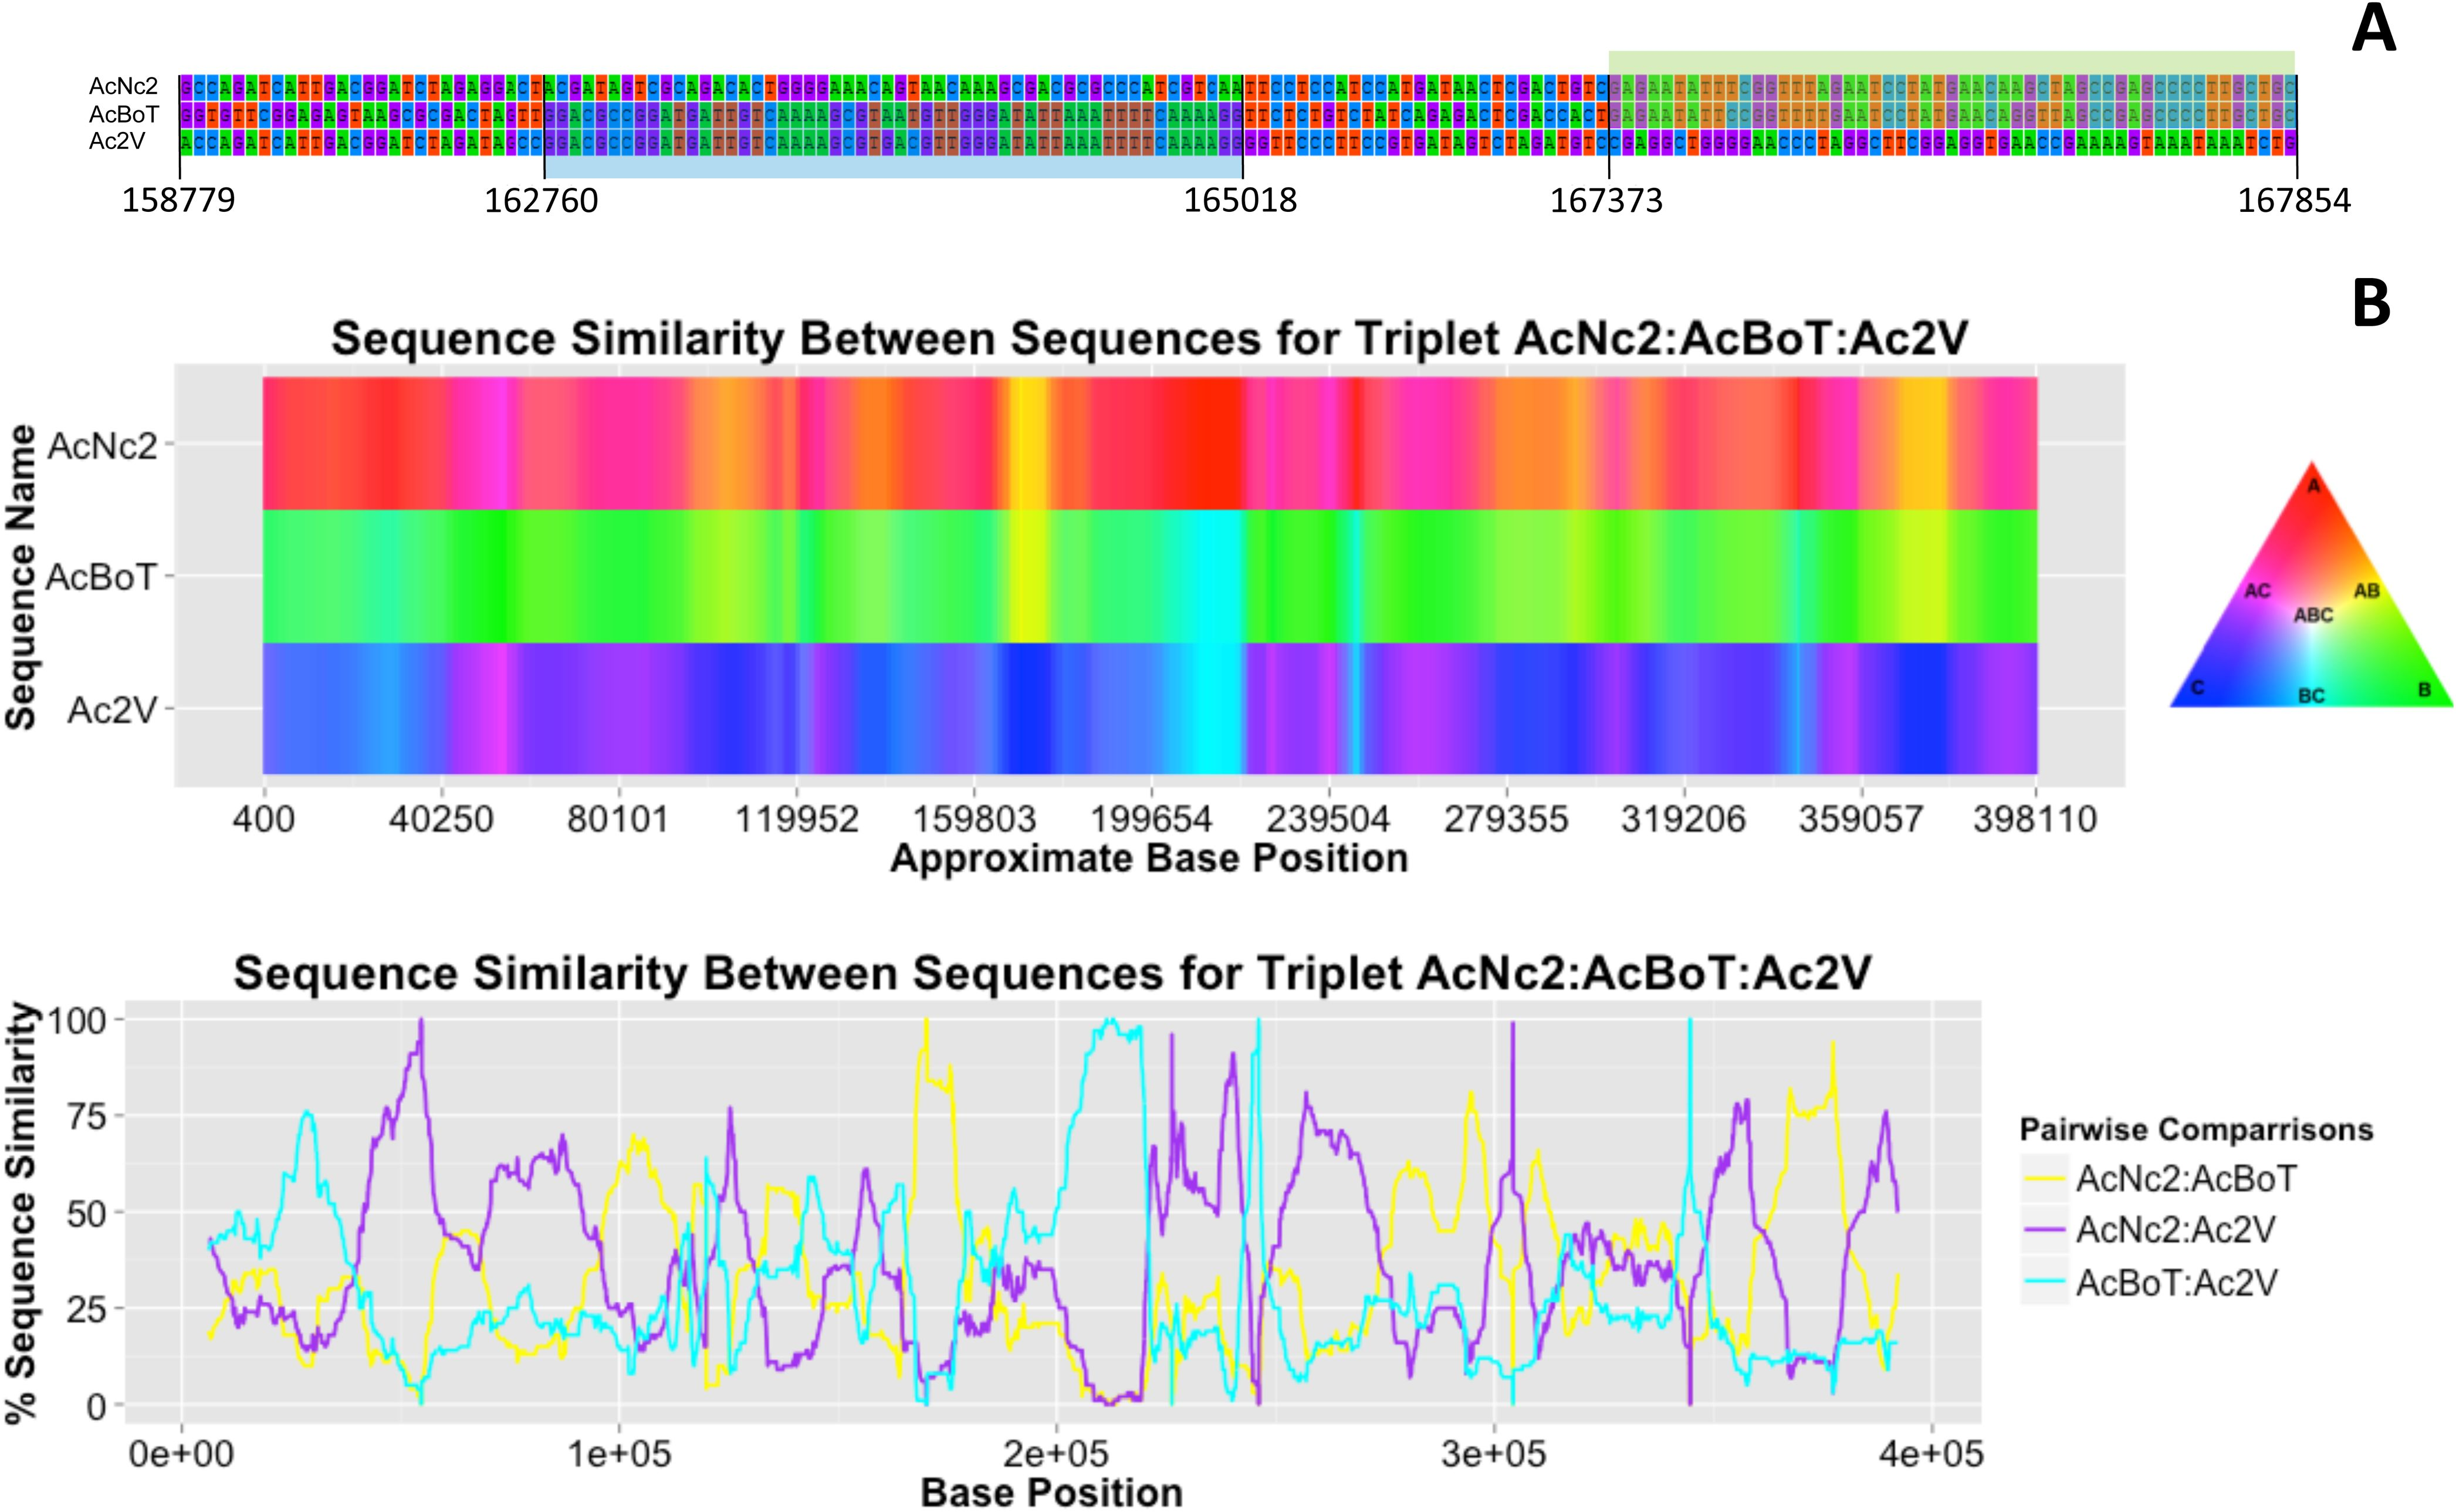
\includegraphics{Figures/AlbugoCandida/AC_Figure2}
\caption{Extensive variation in sequence similarity between \textit{Albugo candida} races.
\textbf{A)} An sequence alignment between base positions 158,779 and 167,382 within contig 1 of \textit{A. candida} races AcNc2, AcBoT and Ac2V. Two recombination blocks coloured blue and green are visible, displaying high sequence similarity between races.
\textbf{B)} The sequence similarity across the length of contig 1, amongst three \textit{A. candida} races. Similarity is visualised using the colours of a RBG colour triangle in the software HybridCheck. Areas where two contigs have the same colour (yellow, purple or turquoise) are indicative of two races sharing the same polymorphisms. The linear plot of the proportion of SNPs shared between the three pairwise comparisons between the races. Shown on the X-axis is the actual base position.\label{fig:AC_Res_2}}
\end{figure}

This observation of alternating blocks of high sequence identity between otherwise diverged (as represented by areas of red, green, and blue) genomes, provides supporting evidence for genetic introgression between diverged races that show a considerable (yet still incomplete) level of reproductive isolation. The recombination detection methods described in the previous section test for recombination blocks visualised here, formally.

\subsection{Recombination blocks identified using RDP}
All 133 contigs were analysed for presence of recombination blocks using algorithms in the software package RDP.
Recombination analysis with these algorithms identified ~675 recombination blocks on 127 sequence contigs which were significant, even following correction of the alpha with a Bonferroni correction.
These identified blocks were reported as significant for at least three different recombination detection tests.
If the length of all the significant blocks is summed in a linear fashion, then approximately 25\% of the total length of all contigs analysed is identified as recombinant, this is equal to 3Mb.
These blocks represent regions of the genome which are derived from either another race, or the ancestor of another race.
Algorithms in RDP were able to report such donor sequences in some cases. 
The full data-set from the RDP output is publicly available from http://dx.doi.org/10.7554/eLife.04550.015.

\subsection{Estimated ages of recombination events}
Dating analysis of the significant recombination blocks using the HybridCheck binomial algorithm indicated that the recombination events detected occurred at a range of different dates. If one assumes a $\mu = 10^{-8}$ substitution rate which is constant across cell cycles, and that there are 100 cell cycles per year, then the most recent introgression event occurred approximately 220 years ago, and the oldest detected event occurred almost 200,000 years ago. The mean age for all the detected recombination events is approximately 6237 years ago, with a standard error of 12,594 years. Furthermore, there is no significant difference between the average estimated dates across different contigs.

The wide range in age estimates of the introgressed regions provides evidence for the hypothesis that recombination and hybridisation between diverging \textit{Albugo candida} races has been a consistent and ongoing evolutionary process, affecting the entirety of the genome. This finding rules-out the hypothesis that one or a few recombination/hybridisation events in the distant past are responsible for creating the mosaic structure observed. This also helps explain the cause of the mosaic genome structure that has been observed: occasional introgression events across a range of evolutionary times is expected to result in genome containing introgressed blocks of sequence from a donor race, interspersed inside the distinct genomic background of the recipient race (i.e. the very pattern observed in \textit{Albugo candida}).

\begin{figure}
\centering
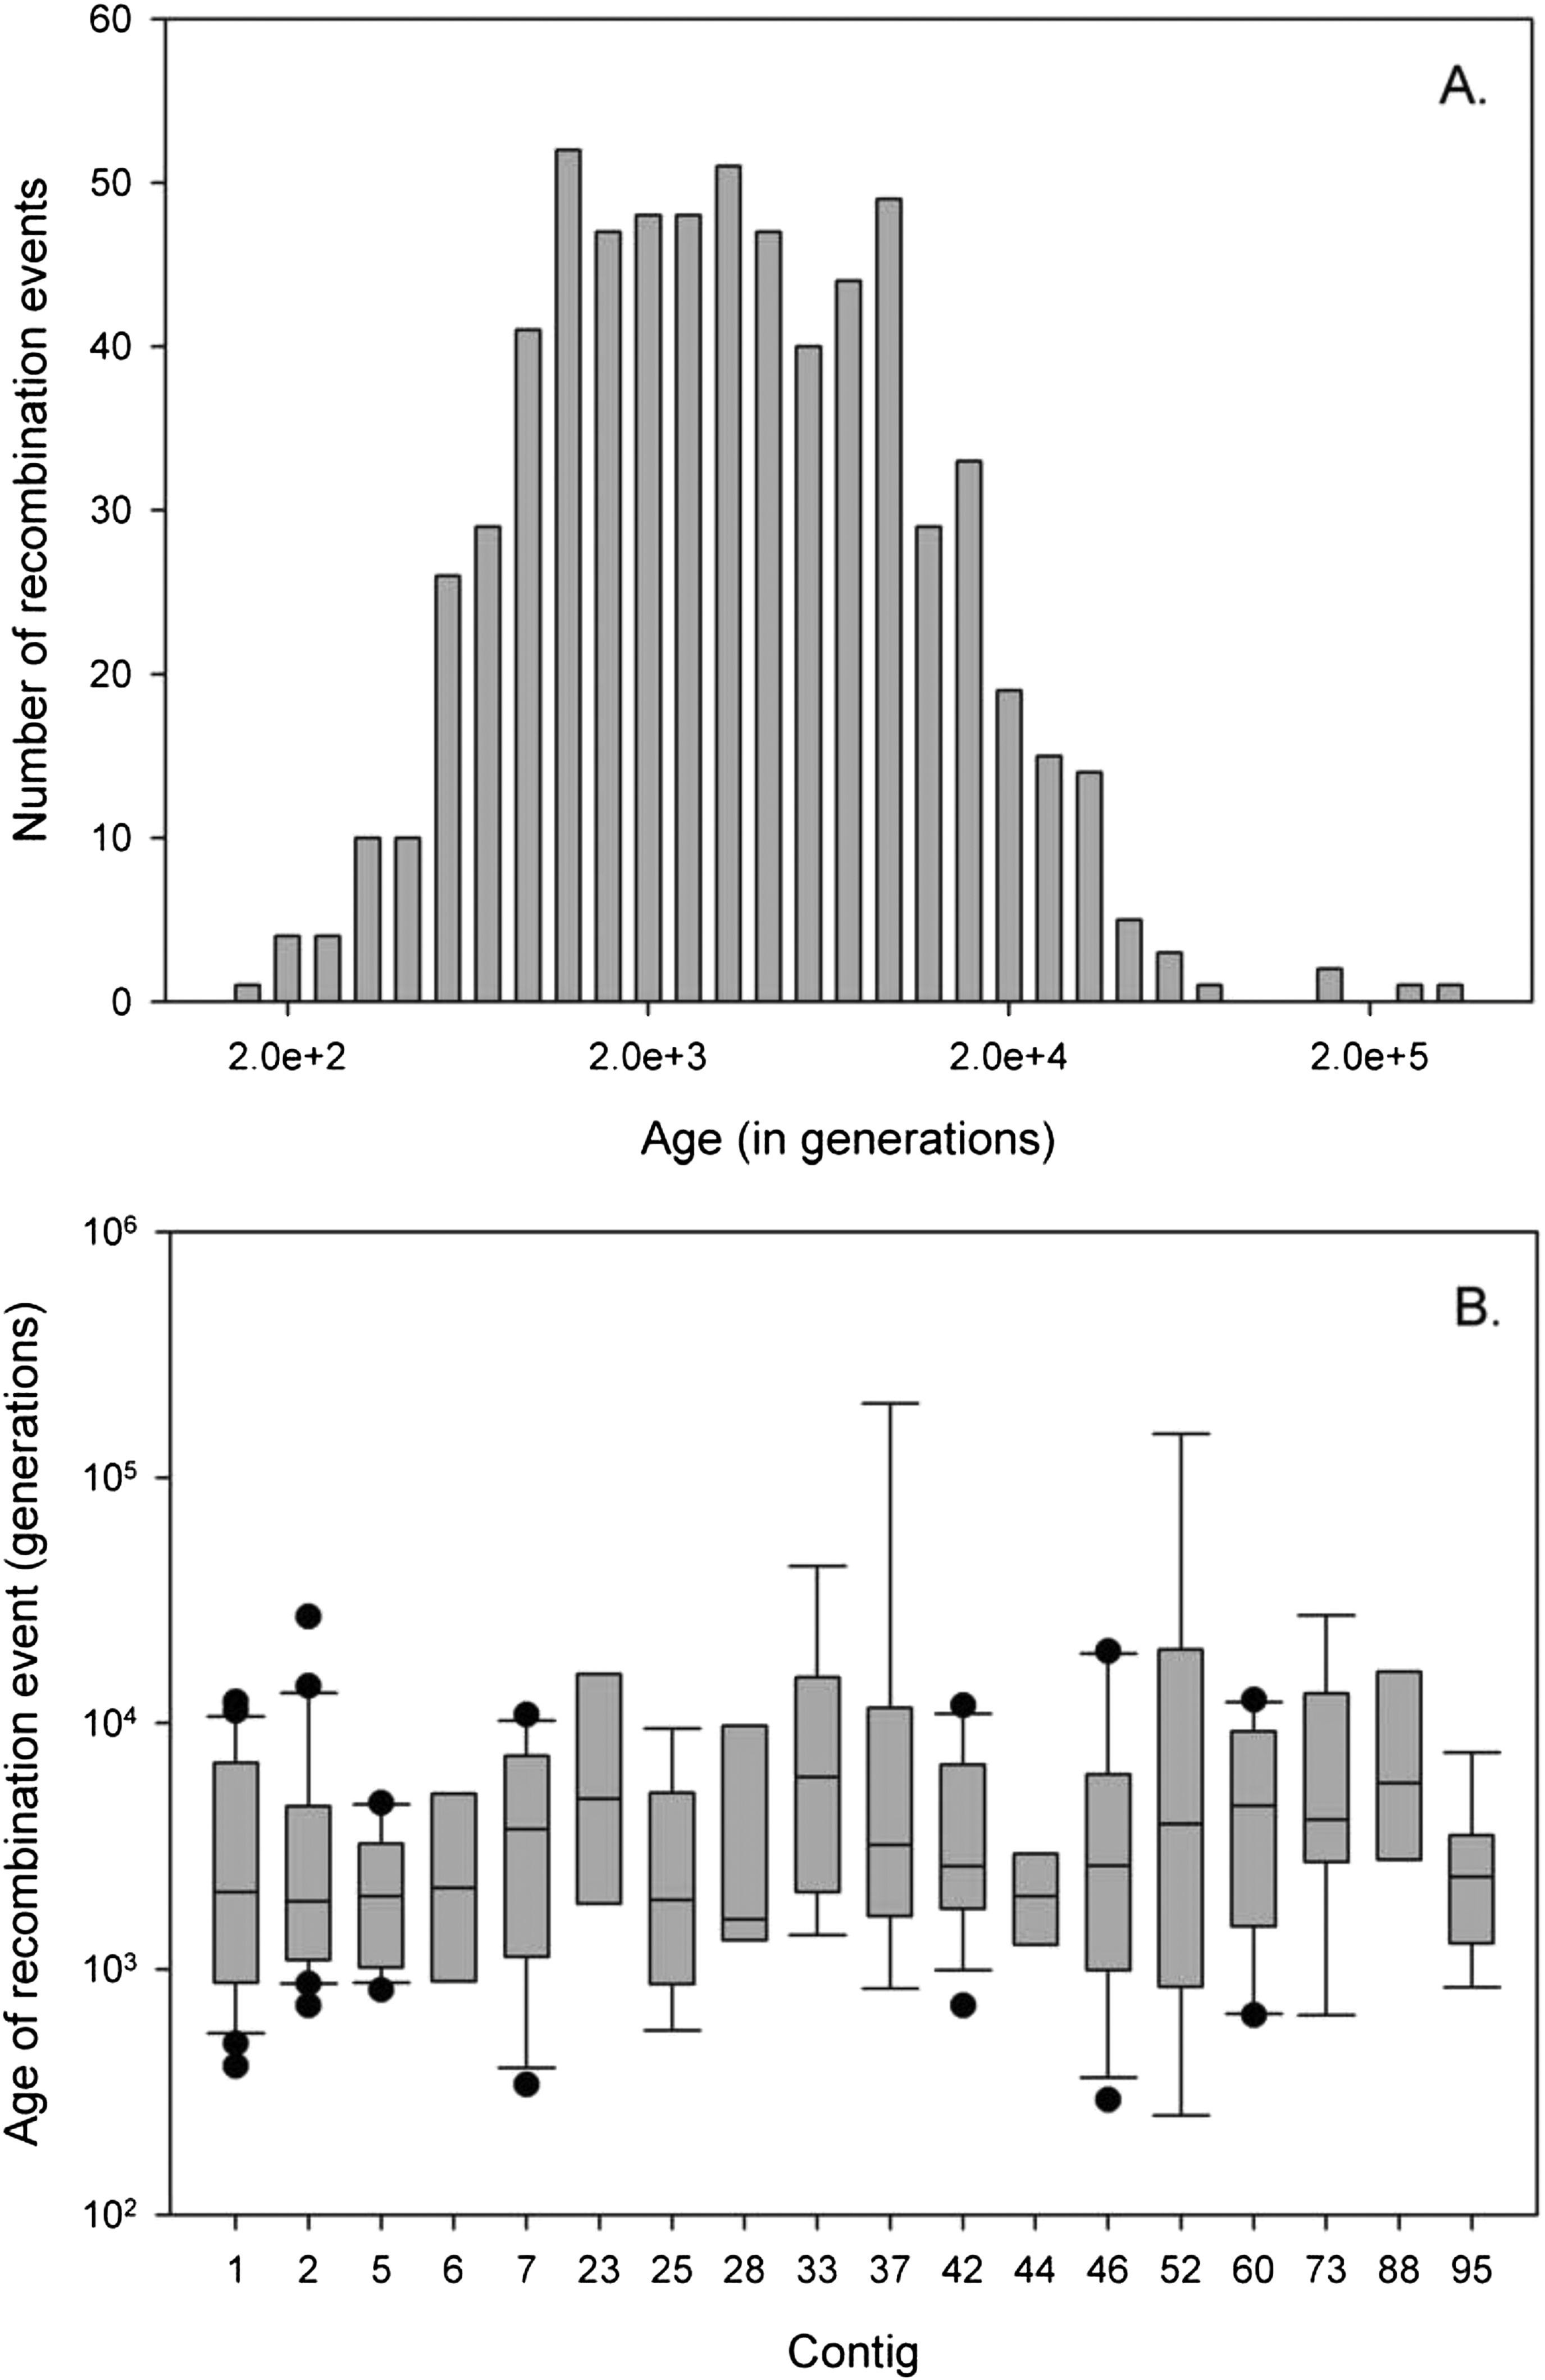
\includegraphics[width=0.7\textwidth]{Figures/AlbugoCandida/AC_Figure3}
\caption{\textbf{A)} Age of the 675 recombination blocks, identified across the whole genome, estimated using the HybridCheck binomial mass function, assuming a substitution rate of $\mu = 10^{−6}$; \textbf{B)} A box plot of the median (plus first nation blocks and third quartile) log-age of recombination events in contigs. Only contigs with eight or more events are shown. There is no significant difference in age of events between contigs (GLM: $F22, 233 = 1.06$, $p = 0.387$).\label{fig:AC_Res_3}}
\end{figure}


\section{Discussion}

The genome of \textit{Albugo candida} appears to have a mosaic-like genome structure: 675 regions were identified in 127 analysed contigs, which were consistently identified by multiple and independent recombination detection methods. 
The mosaic-like structure reflects discordant phylogenetic signals of genomic regions with distinct coalescence, and this suggests that introgression has occurred at a range of time points throughout the evolutionary history of the \textit{Albugo candida} races.

\subsection{Hybridisation and clonal reproduction of \textit{A. candida}}

\textit{Albugo candida} is an obligate biotroph, growing and reproducing on living plant tissue, and virulence experiments confirm that the \textit{Albugo candida} races isolated in this study are indeed host specific \parencite{McMullan2015a}⁠.
To explain the observed mosaic genomes, two distinct and host specialised \textit{Albugo candida} races would have to make contact by colonizing the same host plant in order to hybridize, although ex-situ hybridisation cannot be ruled out. 
Yet, any \textit{Albugo candida} race landing on a non-host plant is likely to trigger host immunity before it can mate with another distinct race.
So, given that the genome structure expected from recent introgression between distinct races is observed, how have they made contact?
One potential explanation was that infected host plants could form secondary contact zones for \textit{Albugo candida}: if a host plant was infected by a compatible (infectious) \textit{Albugo candida} race its immunity would be suppressed.
With a suppressed immune system, non-specialised \textit{Albugo candida} races might be able to colonise the already infected host, enabling both races to make contact and hybridise through sexual reproduction.
This hypothesis was tested with experimental infections of host plants with multiple races.
These experiments confirmed that a virulent race of \textit{Albugo candida} could suppress the immunity of its host plant, such that other non-virulent races of \textit{Albugo candida} could co-colonise it \parencite{Cooper2008,McMullan2015a}.

Following formation of a viable hybrid, clonal reproduction would allow fast dispersal of the pathogen and population expansion.
This aspect of the model was supported by analysing genomic identity between isolates which infect the same host species (i.e. within different races) and quantifying the shared proportion of heterozygous sites.
Genotypic similarity at heterozygous sites of pairs of independent isolates that infect the same host plant was exceptionally high; AcBoT and AcBoL shared 97\% of their heterozygous sites in common, and AcEm2 and AcNc2 shared 99.95\%.
Sharing of this proportion of heterozygous sites rules out Mendelian segregation and sexual reproduction, and confirms that these isolated were reproduced clonally. 
Given that AcEm2 and AcNc2 were sampled 100 miles apart geographically, and ten years apart in time, clonal reproduction appears to be the principal mode of reproduction of this race of agronomically important pathogens. 

The largest contig of the reference assembly, (contig 1; ~400kb) was used to analyse polymorphism distribution and detect recombination blocks.
The proportion of heterozygous sites in contig 1 was calculated for each isolate. 
Very few sites of contig 1 were heterozygous within AcNc2 (0.03\%), AcEm2, and Ac2V (0.01\%).
Within isolates AcBoT and AcBoL, the proportion of heterozygous sites was higher (both 0.65\%).
The high levels of genotypic identity observed between isolates which infect the same the host species would not be expected if sexual reproduction and Mendelian segregation was the primary mode of reproduction, especially given that isolates AcEm2 and AcNc2 are separated by approximately 100 miles and 10 years.
Furthermore, the high proportion of heterozygous sites (for contig 1) in isolates AcBoT and AcBoL is more consistent with asexual population expansion: A diploid organism reproducing asexually/clonally most of the time will accumulate mutations between each pair of homologous chromosomes.
This will generate more heterozygous sites over time, resulting in allelic divergence and increased observed heterozygosity.
However, the observation of a low level of observed heterozygosity in AcEm2 and AcNc2 is not expected in organisms where asexual and clonal reproduction is the primary method of reproduction.
Given there is no evidence of self-fertilisation (or any other form of asexual reproduction), it is likely that gene conversion has been operating to reduce within genome diversity in the races over time.
The phenomenon is called Loss of Heterozygosity or LOH, and it has been observed in other plant pathogen species such as \textit{Phytophthora capsici} \parencite{Lamour2012PathogenCapsici}⁠, as well as at a whole genome scale in yeast \parencite{Diogo2009}.
In both studies it was hypothesized the Loss of Heterozygosity observed has facilitated rapid adaptive evolution and genome plasticity.

To summarise, it appears that the generalist pathogen \textit{Albugo candida} is comprised of distinct physiological races, which are diverging as they specialise on different host species.
Secondary contact between distinct races on an immunosuppresed hosts results in inter-specific sexual reproduction between races, producing new hybrid offspring. 
These hybrids may be able to spread rapidly by clonal reproduction on their own, or introgression may occur.

\subsection{Biology of genetic introgression and hybridisation}
Introgression is defined as the transfer of genetic information (DNA or RNA) from one species (or OTU, race, or biotype) to another as a result of hybridization between them followed by repeated backcrossing \parencite{Ridley2004,Abbott2013}.

Hybridisation and introgression can lead to a mosaic-like genome structure, with regions of different parental lineages interspersed throughout the genome \parencite{Baack2007,Stukenbrock2012}.
Those regions will have different ancestry or coalescence, and hence, be represented by different phylogenetic trees.
Introgression has the potential to augment the adaptive evolutionary potential of populations and introduce a source of genetic variation into genomes.
As a source of genetic variation, mutations have longer waiting times, and lower initial frequencies.
In contrast, introgression can occur multiple times, thereby increasing the probability of fixation of the variant.
Furthermore, whereas mutations tend to be neutral \parencite{Kimura1968EvolutionaryLevel.}, or have (slightly) deleterious fitness effects \parencite{Ohta1973}, introgression inserts “pre-selected” variation of one of the parental (donor) lineages into the hybrid line \parencite{Hedrick2013}.
Adaptive introgressed variants can be new, have less pleiotropy, less strong linked effects, and less recessivity \parencite{Hedrick2013}⁠.
In contrast to mutation, multiple simultaneous changes across multiple loci are possible with hybridisation and introgression, but whether these multiple changes are deleterious or not depends on the details of the molecular interactions within the hybrid.

The view of Wright is that selection favours favorably interacting gene combinations, resulting in a highly integrated genome which contains coadapted gene complexes \parencite{Wright1931,Wright1932TheEvolution,dobzhansky1970genetics}. However, Fisher argued that selection acts on individual genes, and would favour genes which increase fitness on average across all possible genetic backgrounds of a given lineage, such genes were called "good mixers" \parencite{Fisher1930THESELECTION}. Both of these views are compatible with the concept of negative epistasis \parencite{Hedrick2013,Burke2001GeneticsHybrids} in a hybrid genetic background (also called hybrid incompatibility): In any two separated lineages, fixation of alleles in one lineage occurs independently and there is no selection for compatibility with any other lineage. Hybridisation produces novel genotypes which have not previously been subject to selection, and if they are less well adapted than the parental genotypes, selection would act against such less fit hybrids. This reduction in fitness of segregating hybrids has been taken as evidence for unfavorable interactions between genomes of parental individuals, negative epistasis, and hybrid incompatibility. The most widely accepted model of such incompatibility was developed by Bateson, Dobzansky and Muller \parencite{Dobzhansky1936StudiesHybrids.,Muller1942IsolatingTemperature}. Negative epistasis has been confirmed empirically in several animal and plant organisms in the past, including (but not limited to) \textit{Drosophila spp.} \parencite{True1996,Palopoli1994GeneticsStudies,Hollocher1996TheEffects,Cabot1994GeneticsSterility}, \textit{Helianthus spp.} \parencite{Rieseberg1996,Rieseberg1999HybridSpecies}, \textit{Tigriopus californicus} \parencite{Burton1990HybridApproach,Burton1990,Burton1999GeneticComplexes}, and \textit{Iris spp.} \parencite{Cruzan1994AssortativeZone,Burke1998GeneticHybrids}, and is a primary cause of hybrid inferiority.

However, hybrids can be superior to their parental lineages. Hybrid fitness can occur by several means. F1 hybrids are commonly larger in body size and have higher growth rates and yields \parencite{Baack2007,Hedrick2013,Burke2001GeneticsHybrids}. Such vigour is called heterosis, and is explained by the dominance and the over-dominance hypotheses \parencite{Baack2007,Lippman2007}. Other explanations posit that synergistic interactions between different alleles at different loci (i.e. positive epistasis and inheritance of complete co-adapted linkage blocks), and changes in gene expression can also contribute to heterosis \parencite{Baack2007,Swanson-Wagner2006AllParents.}. Heterosis may contribute towards the establishment of an asexual or allopolyploid hybrid. Fitness resulting from Heterosis may be short lived, for introgressed hybrid lineages. This is because sexual reproduction over several generations would cause loss of heterozygosity in the subsequent (backcrossed) generations. Instead, long term success depends largely on the fixation of novel favorable gene combinations from the two parents \parencite{Baack2007,Burke2001GeneticsHybrids}. The genes in such combinations must either interact favorably with other genes in the combination to increase fitness, or ⁠increase fitness in an additive way, with little or no interaction. Thus, selection and niche differentiation play a central role in the establishment of these relatively fit hybrids, because otherwise competition and gene flow with parental populations may overwhelm them \parencite{Buerkle2000TheSpeciation.,Rieseberg1999TransgressiveSpeciation.}. Just as evidence of negative epistasis has been found empirically in several species, empirical evidence of epistasis producing relatively fit hybrids has also been found for several species. For example, in addition to confirming cases of hybrid inferiority in \textit{Helianthus spp.}, Rieseberg and colleagues also found beneficial epistatic interactions in hybrid of \textit{Helianthus annuus} and \textit{Helianthus petiolaris} \parencite{Gardner2000InferringZones,Rieseberg1996}. Evidence of favorable cytonuclear interactions was found in hybrids of \textit{Iris fulva} and \textit{Iris brevicaulis}, indicating that as well as interactions between genes, interactions between the nucleus and the cytoplasm can also determine the success of a hybrid \parencite{Burke1998GeneticHybrids}. Hybrid lineages may also exhibit transgressive segregation i.e. they may have more extreme trait values than either of the parents, when the parents possessed alleles of opposing effects. This may be beneficial or deleterious, depending on the nature of the trait and may be caused by epistasis, or, as QTL analyses have demonstrated, through additive effects \parencite{Baack2007,Burke2001GeneticsHybrids}.
Hybridisation could also help purge mutational load by the masking deleterious alleles in heterotic F1 individuals, followed by introgression of favorable alleles \parencite{Ingvarsson2000HeterosisRate.}.

\subsection{Introgression and evolution of \textit{Albugo candida} in the wider context}

Given the potential advantages of introgression, it has been hypothesised that introgression it is instrumental in generating novel combinations of pre-selected virulence effectors from different diverged races in \textit{Albugo candida} \parencite{McMullan2015a}. Not all such combinations may be successful or viable, but successful genotypes would be important in facilitating the colonisation of new hosts i.e. a host jump. As a hypothetical example, the \textit{Albugo candida} race Ac2V is proposed to possess an effector allele, which interacts with an \textit{Arabidopsis} R gene called WRR4. This prevents Ac2V from colonising \textit{Arabidopsis}. It is unknown which effector interacts with WRR4, but if the effector allele segregated away in hybrid offspring, or was removed through loss of heterozygosity, the hybrid offspring may be able to overcome \textit{Arabidopsis} resistance.

The impact of introgression and hybridisation has been demonstrated in other species. For example, in sunflower species \textit{Helianthus anomalus} \parencite{Ungerer1998RapidSunflowers.}. \textit{Helianthus anomalus}, like \textit{Albugo candida}, has a genome which appears to be composed of distinct parental blocks. However, unlike \textit{Albugo candida}, the introgression was dated as occurring over a short timespan of 10 - 60 generations, which provides support for the idea that hybrid speciation is a punctuated process \parencite{Ungerer1998RapidSunflowers.}⁠. The dating analysis of blocks present in \textit{Albugo candida} suggests that introgression has occurred between different races at different times, and repeatedly throughout the evolution of the species. Furthermore, unlike \textit{Albugo candida}, introgression in the sunflower species occurred between two different species, and resulted in a new hybrid species. For \textit{Albugo candida}, whilst the races are isolated from each other most of the time, repeated introgression between them during secondary contact on immunosuppressed host plants likely acts to prevent them becoming completely isolated, new species. A classic example of an adaptive radiation is Darwin's Finches (\textit{Geospiza}, \textit{Certhidea}, \textit{Pinaroloxias}, and \textit{Camarhynchus/Platyspiza} spp.), and even here hybridisation has been demonstrated \parencite{Lamichhaney2015}: Recent whole-genome resequencing, and phylogenetic analysis based on autosomal, mtDNA, and sex-linked loci of 120 birds representing all of the Darwin finch species and two other related species revealed discordant phylogenies \parencite{Lamichhaney2015}⁠. Calculations of Patterson's D, supported the hypothesis of gene flow and hybridisation throughout the radiation \parencite{Lamichhaney2015}⁠. Rare introgression is thought to have facilitated the exchange of mimicry genes between \textit{Heliconius} butterfly species, post isolation \parencite{Martin2013}.

Studies from hybridisation with yeast provide findings which corroborate the findings of this study. For example, genetic exchange between 3 strains of \textit{Saccharomyces cerevisiae} has been quantified, and indicates that for these strains out-crossing has only occurred 314 times during approximately 16 million cell cycles \parencite{Ruderfer2006PopulationYeast.}. This is approximately one out-crossing event per 50,000 cell cycles. Thus while the strains of yeast do mate and recombine in the wild, this is not a frequent occurrence \parencite{Ruderfer2006PopulationYeast.}⁠. This is also what has been inferred for \textit{Albugo candida} as the result of this study. In addition, the genomes of wine strains of \textit{Saccharomyces cerevisiae} contain introgressed blocks from the species \textit{Saccharomyces paradoxus}, \textit{Saccharomyces kudriavzevii kudriavzevii}, \textit{Saccharomyces uvarum uvarum}, and \textit{Zygosaccharomyces bailii} \parencite{Dujon2010YeastGenomics}⁠. The blocks in the genome of \textit{Saccharomyces cerevisiae} are almost identical to the corresponding regions in the genomes of the donor species, indicating that the introgression events have been recent \parencite{Dujon2010YeastGenomics}⁠. This is similar to what this study has demonstrated for \textit{Albugo candida}. It appears that introgression is a general phenomenon in yeast genomes, but one review concluded that its importance in its evolution has yet to be determined.

The importance of introgression in the evolution of \textit{Albugo candida} is hypothesized to be as follows: Isolation, divergence and specialisation of races will generate repertoires of “tried and tested” effectors for a specific race. Those  adapted race-specific repertoires are then brought together when two races hybridize to generate novel repertoires of novel combinations of these effectors. Specific avirulence effectors that trigger host immunity may be lost through segregation and the “Loss of Heterozygosity” (LOH) effect hypothesized to be taken place in oomycetes by \cite{Lamour2012PathogenCapsici}, and documented here and in \cite{McMullan2015a}. These hybrids, having new combinations of effectors, and having lost effectors which impeded their colonisation of other hosts previously, may expand their geographical range and population size clonally. Such new hybrids may be able to colonise new hosts, explaining the phenomenal host range of species such as \textit{Albugo candida} (and possibly other “generalists”). Hybridisation between races has been shown to expand host range in other plant pathogen species such as \textit{Phytopthora} spp. \parencite{Ersek1995CreationFusion}⁠, and the transfer of virulence genes leading to host range expansion has also been demonstrated in bacterial and fungal pathogens \parencite{FordDoolittle1999LateralGenomics,Mehrabi2011HorizontalRange}. Sexual oospores of \textit{Albugo candida} are tolerant of strong environmental pressures, which raises the prospect: might hybrid spores produced by reproduction between two races lie dormant, forming banks of hybrid genotypes, waiting for conditions better suited to their genotype and phenotype?

The ability to expand host range and generate novel genotypes through hybridisation, and then reproduce rapidly clonally may be especially favored in a monoculture based agro-ecological environment, characterized by different, large, homogeneous regions of (often clonal) host plants of one species \parencite{Stukenbrock2012AAgro-Ecosystems}⁠. Recently \cite{Stukenbrock2012}⁠ demonstrated that the plant pathogen species \textit{Zymoseptoria pseudotritici} was formed by the hybridisation of two distinct fungal individuals, and that the genome is characteristic of bottleneck and selection following the hybridisation event which occurred approximately 380 sexual generations ago, resulting in the generalist grass pathogen. The obligate biotroph and powdery mildew, \textit{Blumeria graminis f. sp. Hordei} also has a mosaic genome of alternating monomorphic and polymorphic DNA sequence blocks \parencite{Hacquard2013MosaicHosts.}. Pathogen adaptation to agro-ecological environments is characterized by high genome plasticity of pathogens (a successful pathogen needs to keep up in the co-evolutionary arms race with its host), but a reduction in diversity for recently emerged lineages (selection is strong and new and recently emerged lineages are often bottlenecked) \parencite{Stukenbrock2012AAgro-Ecosystems}⁠. Pathogens such as late blight of potato, \textit{Phytophthora infestans}, wheat yellow rust \textit{Puccinia striiformis}, and \textit{Magnaporthe oryzae}, which are specialised, may represent an end-result of a much broader process of pathogen adaptation and evolution. The results gained from this work provide insight into how recombination and hybridisation plays a role in generating novel virulent races, and into their subsequent spread and geographical range expansion by clonal propagation. These findings are of particular relevance to modern, monoculture based agriculture.  
